\chapter{Introduction}

AlphaFlow is an activity-based workflow engine for Plone. It manages tasks to
be performed on content objects. Outstanding features of AlphaFlow are:
\begin{itemize}
    \item a simple workflow definition format
    \item reusable components with exhaustive standard library including
        task assignments, decisions, scripting, email notifications, time based triggers, recursive publication, and more.
    \item easy modelling of complex workflows thanks to decentralized flow
      control
    \item individual workflows for each content object
    \item parallel workflows
    \item flexible management of user assignments as well as permission and
      role mappings for content objects and tasks
\end{itemize}

AlphaFlow is not the only workflow engine available for Zope/Plone. There are two
others:
\begin{itemize}
\item ``DCWorkFlow``, a state-based workflow engine, created at Zope Corporation for use with the CMF.
    DCWorkFlow is integrated into Plone by default.
\item ``OpenFlow'', a general purpose activity-based workflow engine for Zope.
\end{itemize}

Having used DCWorkFlow for a long time and having studied the concepts of
OpenFlow, we are very grateful for those open source systems. AlphaFlow was
built to overcome certain limitations of both engines, but was also build with
the good experiences of DCWorkFlow and OpenFlow in mind.

\section{About this document}

This document is intended to help you get started with AlphaFlow.  It provides
\begin{itemize}
    \item tutorials on how to get started using AlphaFlow and developing with AlphaFlow
    \item an architectural overview
    \item API and library references 
    \item some recipes on standard workflow patterns
\end{itemize}

\section{Terminology}

A real-world workflow is described to AlphaFlow by a ``workflow definition''.
A workflow definition, like a real-world workflow, consists of several steps
which we call ``activities''.

Every time a defined workflow is started, a ``workflow instance'' is created.
The workflow instance runs a series of ``work items''. Each work item
corresponds to an activity. Work items follow up on each other as described by
the workflow definition.

\begin{figure}
  \centering
  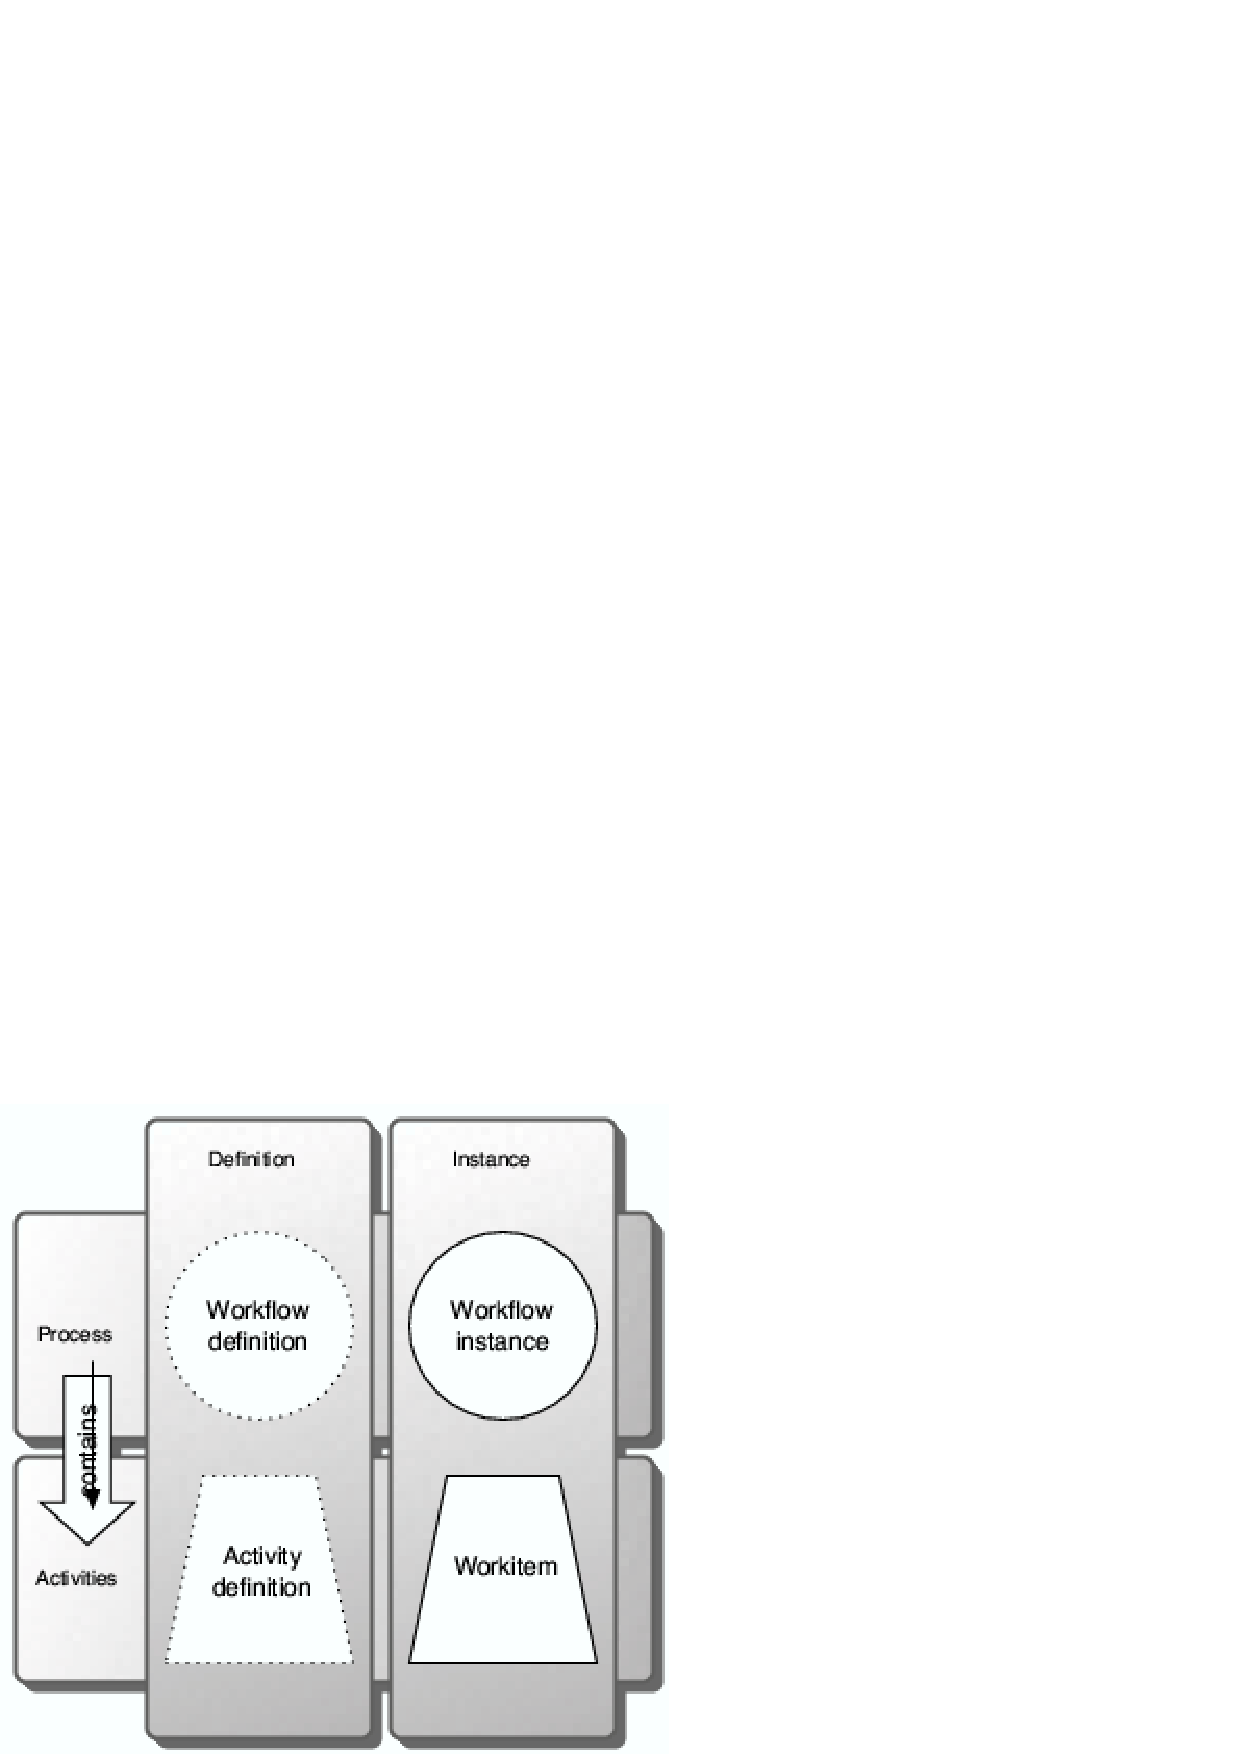
\includegraphics{terminology}
  \caption{\label{fig:terminology}%
    Relationships between a workflow, its definition, and the steps they
    consist of.}
\end{figure}
